%!TEX root=Principal.tex
\chapter{PROJETANDO TESTES EM INTERAÇÃO HUMANO-ROBÔ}
\label{cap:projetoihr}
Esse capítulo é dedicado a toda fase de preparação para os testes e estudos em Interação Humano-Robô~(IHR). É apresentado um conjunto de variáveis e como foram selecionadas para o teste de objetivo específico na interação. Quais são os fatores de projetos que devem ser considerados, preparação do robô e do ambiente, definição do contexto de uso. A execução do experimento e como é coletada cada informação sobre a IHR. Análise dos primeiros resultados obtidos para criação de um mecanismo probabílistico que auxilie na classificação do usuário. Todos esses pontos estão ilustrados na figura~\ref{fig:experimento}.

\begin{figure}[ht!]
	\centering
	\begin{minipage}{\textwidth}
		\caption{Visão geral sobre o projeto de IHR desenvolvido.}
		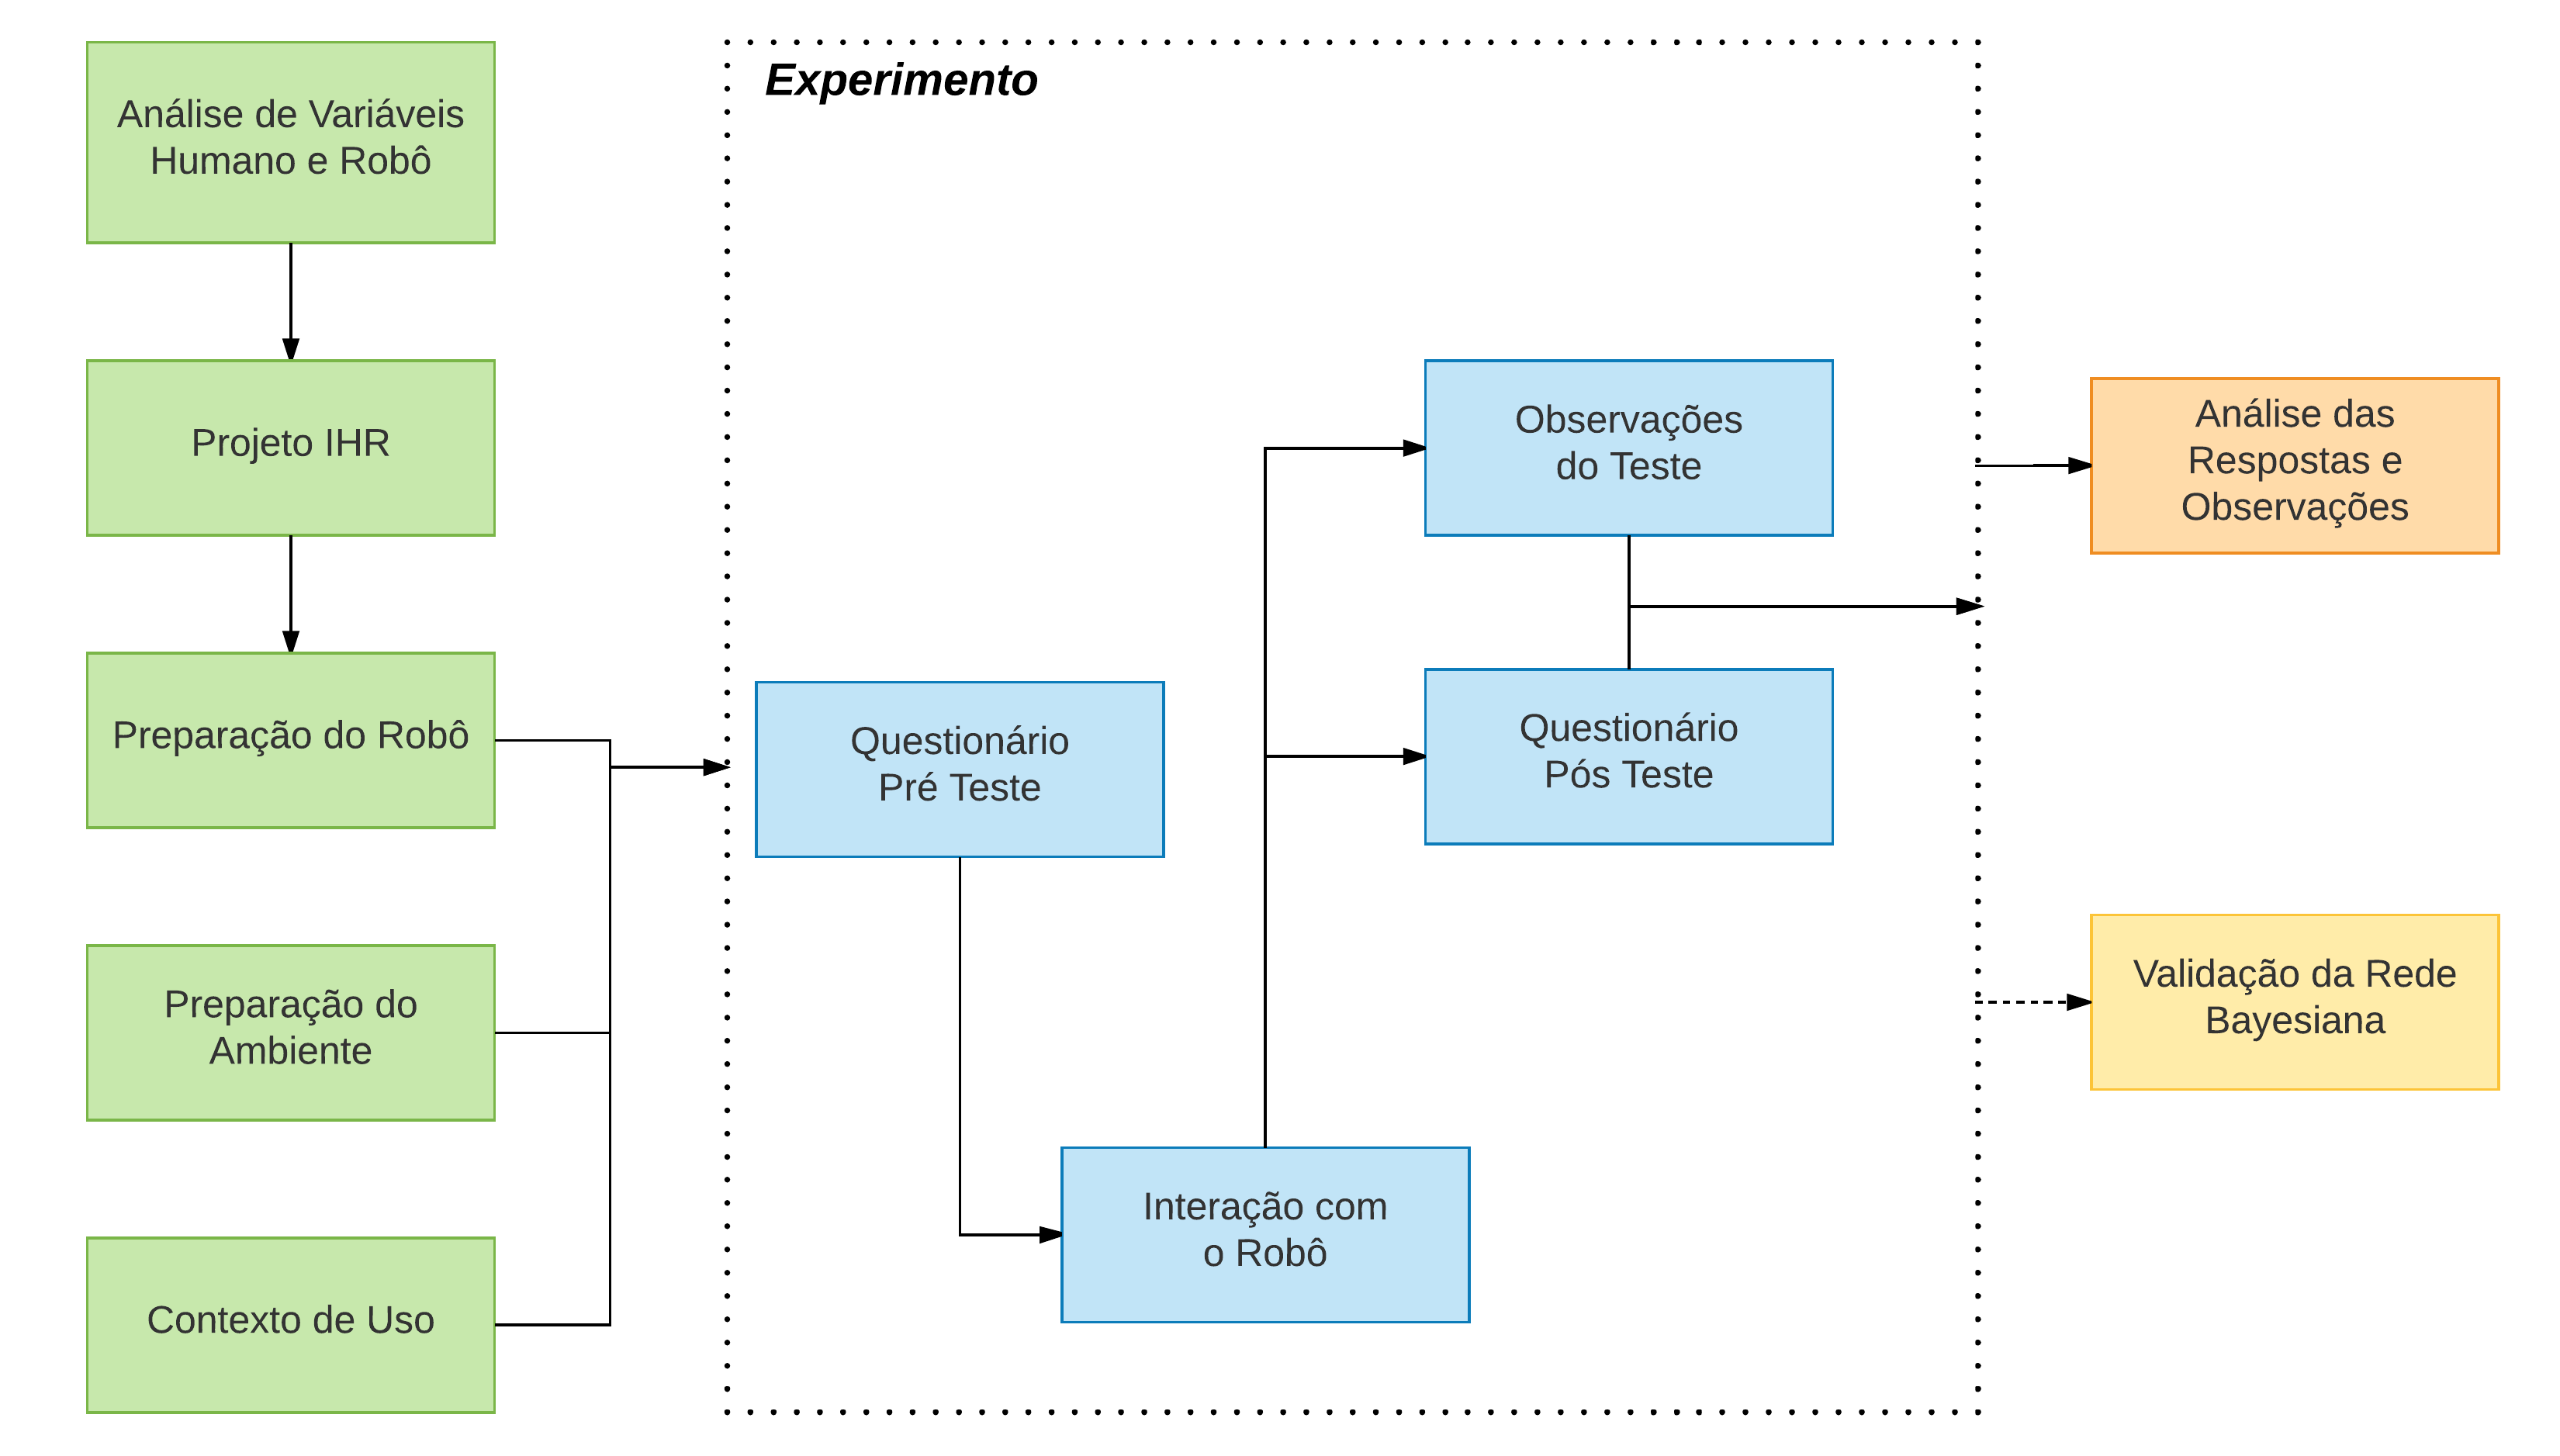
\includegraphics[width=\textwidth]{experimento.png}
		\smallcaption{Fonte: o autor.}
		\label{fig:experimento}
	\end{minipage}
\end{figure}

A figura~\ref{fig:experimento} apresenta a sequência de passos executadas para a concepção do experimento dessa tese. Os primeiros passos auxiliam a definir o escopo do teste e o que será avaliado ao longo do experimento. Esses primeiros passos estão definidos através da cor verde. Em cor azul, estão os passos realizados para execução do teste de interação entre o robô e o ser humano. Por fim, temos duas etapas em tons amarelo e laranja. O amarelo corresponde aos testes de validação do classificador bayesiano e serão discutidos no capítulo~\ref{cap:proposta}. A etapa laranja é referente a análise do especialista após a coleta de informações no teste de IHR. A seguir, cada uma das etapas será discutida e apresentada ao longo do capítulo separadas em seções.

\section{Análise de Variáveis para IHR}
\label{sec:variáveis}
O primeiro passo para construir o experimento é identificar o conjunto de variáveis que possam auxiliar a identificar informações sobre a IHR. Essas variáveis devem ser separadas em classes de maneira que seja possível referência-las em outros momentos do projeto. Além da referência, as classes são importantes pois, ajudam a definir o tipo de projeto que será investigado durante o experimento. A investigação tem o objetivo de melhorar a IHR sempre com o foco nas necessidades do ser humano, o usuário do sistema. Cada classe de variáveis adotada possuí um método diferente para obtenção das informações. Contudo, esse método de captura não é restrito e podem ser discutidos diferentes meios de obtenção da informação. Por exemplo, a variável nome do usuário, pode ser obtida através da interação por voz com o usuário ou através de questionário. O meio de obtenção dependerá do momento e objetivo do experimento.

Para selecionar as variáveis, é realizado um trabalho de revisão bibliográfica e identifica-se como representar as informações necessárias ao problema. Na aproximação do robô, algumas variáveis foram identificadas ao longo do capítulo~\ref{cap:proxemics}. O uso da teoria de proximidade torna possível a extração de fatores comportamentais com base na distância social entre a pessoa e o robô. Esses fatores podem variar não só entre a posição física dos dois agentes, mas também na posição do corpo dos indivíduos, como por exemplo, a orientação dos ombros e troco em relação a posição do robô (linguagem corporal)~\cite{mead:2016}. Outro fator significante é a fixação entre olhares, este pode auxiliar no processo que determina o início e o fim de uma interação. O olhar também auxilia a determinar quem são os principais indivíduos na interação~\cite{mumm:2011, srinivasan:2012}. Pode-se empregar o reconhecimento de expressões faciais para auxílio na análise do quanto a situação é confortável para o indivíduo, ou o quanto o usuário aprecia a interação. Existir uma avaliação em tempo real das reações deste indivíduo durante todo o processo de interação, auxilia na compreensão da experiência do usuário~\cite{amaral:2014}. Outra técnica para análise de conforto na interação é a avaliação da emoção através da voz da pessoa, ou através do uso de equipamento de eletroencefalografia~(EEG), porém este último é um método mais invasivo já que exige a adição de um equipamento na pessoa que interage com o robô~\cite{bos:2006, lee:2014}.

É possível empregar diversos sensores que auxiliam a leitura e quantificação dessas variáveis. Sensores de captura de marcações de movimento, como Microsoft\textregistered\ Kinect\textregistered\ ou o ASUS\textregistered\ Xtion\textregistered, são utilizados para quantificar os valores comportamentais obtidos através das variáveis, que envolvem distância entre agentes e orientação de membros do indivíduo. Para realizar o reconhecimento de expressões faciais utiliza-se uma câmera de video, podendo assim executar uma leitura da face da pessoa em tempo de execução. As variáveis referentes a questão da fixação dos olhares dos agentes para identificar o início e o fim da interação, podem ser obtidas através de ambos sensores, sendo possível determinar a orientação da cabeça e torso do indivíduo, além de também a direção do olhar da pessoa para o robô. A voz do indivíduo para análise da emoção na interação é obtida através de um microfone direcional ou um arranjo de microfones, que amplifica a capacidade de percepção do robô em relação ao ambiente e a pessoa que interage com ele.

As variáveis aplicadas ao comportamento tem dependência do cenário de interação, porém as informações das variáveis etnográficas como idade, experiência computacional, sexo, local de origem, etnia, entre outras, são independentes do cenário. Existem alguns algoritmos na área de visão computacional que são capazes de identificar algumas variáveis etnográficas de maneira automática \cite{yang:2007, shan:2012, ylioinas:2012, samadi:2013, amaral:2014}, isso pode auxiliar no processo de expansão da rede bayesiana de maneira automática. Porém, nem todas as informações podem ser obtidas de maneira automática, então alguns métodos como questionários e entrevistas são necessários para melhor compreendimento do comportamento do usuário e identificar como foi sua experiência durante a interação.

Cada uma das variáves será discutida conforme apresentadas nas seções a seguir.

\subsection{Variáveis Etnograficas}
\label{sec:etnograficas}
As variáveis etnográficas tem o objetivo de coletar informações sobre etnia, cultura, costume e outros fatores antropológicos~\cite{borges:2005}. Além dessas informações, esse tipo de variável auxilia na identificação de dados sobre idade, gênero, experiência social e também tecnológica do indivíduo. Todas as informações representadas nos dados etnográficos são relevantes para verificar a adesão do usuário sobre tecnologias novas, qual cultura ele está inserido, e outras informações que podem determinar o nível de interação que ele aceita. Essas informações podem ser capturadas através de questionários e entrevistas. Caso seja uma necessidade do projeto, o robô pode realizar a entrevista para coletar essas informações. Para o desenvolvimento dessa tese, como essas informações são para analises do especialista, optou-se pela coleta através do questionário. A lista apresentada a seguir define as variáveis etnográficas e uma breve explicação sobre o significado de cada uma.

\begin{enumerate}
	\item \textbf{Idade}: informa a idade do indivíduo.
	\item \textbf{Gênero}: informa o sexo biológico do indivíduo.
	\item \textbf{Local de Nascimento}: informa qual o local de nascimento do indivíduo. Essa variável auxiliará a determinar a base cultural do indivíduo.
	\item \textbf{Etnia}: informa a origem da família do indivíduo. Outra variável que auxilia na determinação da base cultural do indivíduo.
	\item \textbf{Quantidade de \emph{Gadgets}}: informa a quantidade de \emph{gadgets} que o indivíduo possui, ajudando a identificar qual a experiência e o contato dele com a tecnologia.
	\item \textbf{Contato prévio com Robôs}: informa apenas se o indivíduo já possuiu algum contato com robôs. Auxiliará a determinar o contato com a tecnologia, principalmente com robôs que poderá influenciar no seu comportamento durante a interação.
	\item \textbf{Tipos de Robôs}: informa quais são os tipos de robôs que o indivíduo teve contato. Os tipos poderão ser robôs \emph{Pet}, Humanoides, Androides, Móveis, entre outros. Essa variável é um complemento da variável ``Contato prévio com Robôs''.
	\item \textbf{Quantidade de cidades visitadas}: informa a quantidade de cidades que o indivíduo já visitou além da sua cidade natal. É importante para identificar o contato com outros tipos de cultura. Isso poderá influenciar no comportamento definido por sua cultura.
	\item \textbf{Quantidade de cidades que morou}: informa a quantidade de cidades que o indivíduo já morou além da sua cidade natal. É importante para identificar a vivência com outros tipos de cultura. Isso poderá influenciar no comportamento definido por sua cultura.
	\item \textbf{Quantidade de países visitadas}: informa a quantidade de países que o indivíduo já visitou além da sua cidade natal. É importante para identificar o contato com outros tipos de cultura. Isso poderá influenciar no comportamento definido por sua cultura.
	\item \textbf{Quantidade de países que morou}: informa a quantidade de países que o indivíduo já morou além da sua cidade natal. É importante para identificar a vivência com outros tipos de cultura. Isso poderá influenciar no comportamento definido por sua cultura.
\end{enumerate}

Em diversos trabalhos da seção \ref{sec:proxemicsihr}, onde a questão cultural do indivíduo é abordada, são discutidos que influência a cultura provê sobre o comportamenteo do o indivíduo. A cultura é tratada como a origem do indivíduo~\cite{eresha:2013}. Entretanto, a questão cultural na vida de uma pessoa é mais abrangente pois, pode ser relacionada com a experiência adquirida ao longo de sua vivência social, como por exemplo, países e cidades que o indivíduo visitou e viveu, o meio ao qual ele está inserido, sua profissão, entre outras informações. Dessa forma, o conjunto de variáveis apresentado na lista acima auxilia a mapear de forma abstrata a experiência social do indivíduo. O intuito do uso das informações etnográficas é investigar até que ponto elas podem influenciar na experiência do usuário durante a interação com o robô.

\subsection{Variáveis Comportamentais}
\label{sec:reacoes}
Variáveis comportamentais tem como principal objetivo identificar reações de comportamento dentro do cenário exigido por uma determinada tarefa. As variáveis comportamentais são coletadas a partir de informações sobre expressões corporais, expressões faciais e também de declaração explicita da pessoa ou do robô. O uso dessa classe de variáveis possibilita uma análise baseando-se em teorias de linguagem corporal e de microexpressões. Algumas possibilidades para analisar expressões corporais são discutidas no trabalho apresentado por \citeonline{lambert:2008}. O conjunto de variáveis comportamentais apresentados nessa seção podem ser utilizados não apenas para extrair o perfil do indivíduo, mas também para avaliar a ação realizada pelo robô ao interagir com o usuário. Dependendo do \emph{hardware} utilizado no robô, essas variáveis também possibilitam que o robô realize esses comportamentos durante a interação. A lista apresentada a seguir define as variáveis comportamentais obtidas através da literatura e uma breve explicação sobre o objetivo de cada uma das variáveis.

\begin{enumerate}
	\item \textbf{Expressões Faciais}: é possível identificar se a reação do indivíduo foi positiva ou negativa, a partir de uma ação do robô. Existem seis expressões bases que combinadas formam diversas outras~\cite{bihan:2014}. Contudo, nesse trabalho será considerado apenas as seis expressões bases classificadas em dois grupos: expressões faciais positivas e expressões faciais negativas. O intuito dessa variável é realizar a avaliação da ação do robô com base nas expressões faciais do indivíduo.
	\item \textbf{Tempo de Transição entre as Zonas Sociais}: identificar o tempo que o indivíduo ficou confortável com a presença do robô a medida que esse diminuiu a distância entre eles.
	\item \textbf{Frequência do Olhar em direção ao Robô}: identificar se o indivíduo mantém o olhar ao robô, sendo possível saber se a interação está continua ou não. Isso pode influenciar se o robô está interagindo de maneira confortável ao indivíduo ou se esse está incomodado com a presença do robô.
	\item \textbf{Tempo do Olhar}: é possível mensurar o interesse do indivíduo durante a interação através do tempo que ele permanece com o olhar fixo no robô. Quanto maior o tempo do olhar, maior o interesse na interação do indivíduo.
	\item \textbf{Orientação dos ombros}: Auxilia a mensurar o interesse do indivíduo durante a interação, analisando se os ombros possuem a mesma orientação que a cabeça e também uma orientação em direção ao indivíduo que interage com o robô. Além disso, é possível determinar através do alinhamento do quadril com o ombro do indivíduo o ângulo de inclinação de seu torso. A inclinação do torso auxilia a identificar o interesse do indivíduo na interação, para isso basta verificar se ele está inclinado em direção ao robô para determinar um interesse positivo.
	\item \textbf{Orientação do quadril}: Auxilia a mensurar o interesse do indivíduo durante a interação. A orientação do quadril em direção ao robô ou na direção oposta auxilia a determinar o grau de interesse do indivíduo na interação. Quando mais alinhado à direção do robô, maior o interesse do indivíduo na interação.
	\item \textbf{Estilo da Voz}: é importante, pois pode determinar a reação que o indivíduo terá após a interação via áudio com o robô. Além disso, é possível determinar se o indivíduo está confortável ou não durante a interação, analisando o tom de sua voz ao responder o robô. Nesse trabalho, será considerado somente o canal de resposta ao indivíduo.
    \item \textbf{Conforto}: determina se o indivíduo está disposto a continuar a interação ou se algo o incomoda, fazendo com que desista de interagir com o outro agente. Essa é uma informação que pode ser obtida através das demais apresentadas acima ou declarada diretamente pelo usuário, como no caso do projeto desta tese.
    \item \textbf{Medo}: determina se o indivíduo sente-se seguro durante a interação com o outro agente. Pode impactar diretamente a experiência de interação do usuário. Essa é uma informação que pode ser obtida através das demais apresentadas acima ou declarada diretamente pelo usuário, como no caso do projeto desta tese.
\end{enumerate}

As variáveis apresentadas acima podem auxiliar na descoberta do interesse em relação a interação. Algumas delas, como as que envolve o olhar, podem necessitar de equipamentos mais específicos para obter uma melhor acurácia na captura. Outras variáveis necessitam de técnicas e estudos direcionados para trazer a interação à um nível mais natural, como o caso da voz. Dessa forma, escolher quais variáveis trabalhar tem influência não só sobre o estudo realizado, como também nos equipamentos embarcados no robô. Tais equipamentos, podem influenciar em sua aparência e consequentemente na experiência do usuário.

\subsection{Variáveis do Robô}
\label{sec:variaveisrobo}
Além das variáveis referentes etnográficas e comportamentais, deve-se considerar também as informações sobre o robô uma vez que sua aparência pode influenciar na reação e expectativa das pessoas durante a interação~\cite{hegel:2009}. Variáveis do robô podem auxiliar a identificar quais são os principais fatores que tornam a interação humano-robô uma boa experiência ao usuário e também natural. Um conjunto de variáveis é apresentado com o objetivo de caracterizar fatores do robô, referente a sua aparência, que influenciam na interação social. Esse conjunto de variáveis é apresentado a seguir:

\begin{enumerate}
	\item \textbf{Altura}: A altura do robô para identificar a influência da diferença entre alturas de robôs e humanos.
	\item \textbf{Volume}: O volume ocupado pelo robô pode influenciar no conforto da interação, uma vez que quando o robô atingir uma zona social mais próxima do indivíduo pode causar uma sensação claustrofóbica a ele.
	\item \textbf{Tipo do Robô}: Segundo \citeonline{choi:2014}, robôs possuem dois tipos: Autônomos e Tele-operados. Essa variável define o quanto de intervenção humana é necessário para que o robô possa executar a tarefa objetivo.
	\item \textbf{Classificação do Robô}: Segundo \citeonline{dobra:2014} classificar um robô é uma tarefa muito complexa e pode envolver diversas variáveis. Dessa forma, para essa tese será considerado uma classificação mais simples. O robô deve ser classificado como: fixo, móvel com rodas, móvel bípede, móvel quadrupede, móvel com manipuladores. Outras classificações podem ser inseridas conforme a necessidade e inclusão de novos robôs.
	\item \textbf{Aparência Física}: Essa variável descreve se o robô possui uma aparência amigável ou agressiva.
	\item \textbf{Nível de Ruído}: Determina qual o nível de ruído que os atuadores do robô podem gerar de tal forma, que possa influenciar na interação humano-robô. Como exemplo, pode-se citar o Big Dog~\footnote{http://www.bostondynamics.com/robot\_bigdog.html}, da Darpa Robotics, que é movido através de um motor diesel e seus atuadores pneumáticos e hidráulicos apresentam um alto grau de ruído.
\end{enumerate}

\subsection{Variáveis de Ações na Interação}
\label{sec:acoes}
Existem variáveis que determinam as possíveis ações que o robô e o ser humano podem executar. Essas ações podem gerar comportamentos diferentes de acordo com o contexto ao qual o cenário está inserido. No caso do robô, as possíveis ações são determinadas a partir do \emph{hardware} disponível para o projeto. Fatores como tipo de manipulador, sonorização, saída de vídeo, entre outros, determinam quais são as ações que o robô deve ter. As variáveis que compõem as informações do perfil comportamental do robô são:

\begin{enumerate}
	\item \textbf{Aproximação}: Forma de aproximação do robô ao indivíduo. Pode ser classificada entre rápida, devagar, brusca ou suave.
	\item \textbf{Movimentação do Manipulador}: Caso exista um manipulador deve descrever como é feita a movimentação do manipulador em direção ao usuário. A classificação pode ser feita entre brusca e suave; ou em relação a sua amplitude, como longo e curto.
	\item \textbf{Estilo de Voz}: Ao emitir algum tipo de som o robô deverá manter um estilo de voz para que seja possível simbolizar qual o tipo de mensagem ele deseja falar. A classificação será feita de maneira simplificada, considerando apenas se é um estilo educado ou agressivo.
	\item \textbf{Volume de Voz}: Ao emitir um som, o robô deve saber qual o volume adequada considerando a interação, ambiente e distância do segundo agente. Uma classificação simples pode ser utilizada, como por exemplo, alto e baixo.
	\item \textbf{Expressão Facial}: Ao iniciar o contato visual com o indivíduo, pode ocorrer diversas expressões do robô na tentativa de manter o conforto do indivíduo durante o processo de interação. Simplificando as expressões são consideradas apenas dois tipos de expressões realizadas pelo robô: amistoso e não-amistoso. As expressões faciais do robô serão executadas através do \emph{tablet} acoplado nele, conforme descrito na seção~\ref{sec:robo}.
\end{enumerate}

A partir das variáveis identificadas, deve-se realizar a definição do contexto de uso, do ambiente e também do robô que serão utilizados no projeto para definir quais e como são utilizadas cada uma das variáveis no projeto de IHR proposto por essa tese.

\section{Contexto de Uso}
\label{sec:contextouso}
Para que a interação com o sistema seja de melhor qualidade, um ponto importante do projeto é definir o contexto de uso. Ele determina quando e onde será realizado a interação com o sistema, no caso desta tese, o robô. O contexto de uso é importante, pois pode influenciar no tipo de comportamento e expectativa do usuário para com o sistema~\cite{barbosa:2010}.

A definição do contexto de uso é baseada em um texto descritivo que delimita todo o cenário da aplicação e como foi planejado o experimento. Esse cenário descreve quem é o usuário, quais os pontos de interação com o sistema e também como será o comportamento do usuário e também do robô. O contexto descrito delimita todo o escopo do teste. Ele assegura que as observações tenham o objetivo de garantir a qualidade do uso dentro daquele cenário. A figura~\ref{fig:contextouso} apresenta o cenário aplicado no contexto de uso dessa tese.

\begin{figure}[ht!]
	\centering
	\begin{minipage}{\textwidth}
		\caption{Ilustração do contexto de uso}
		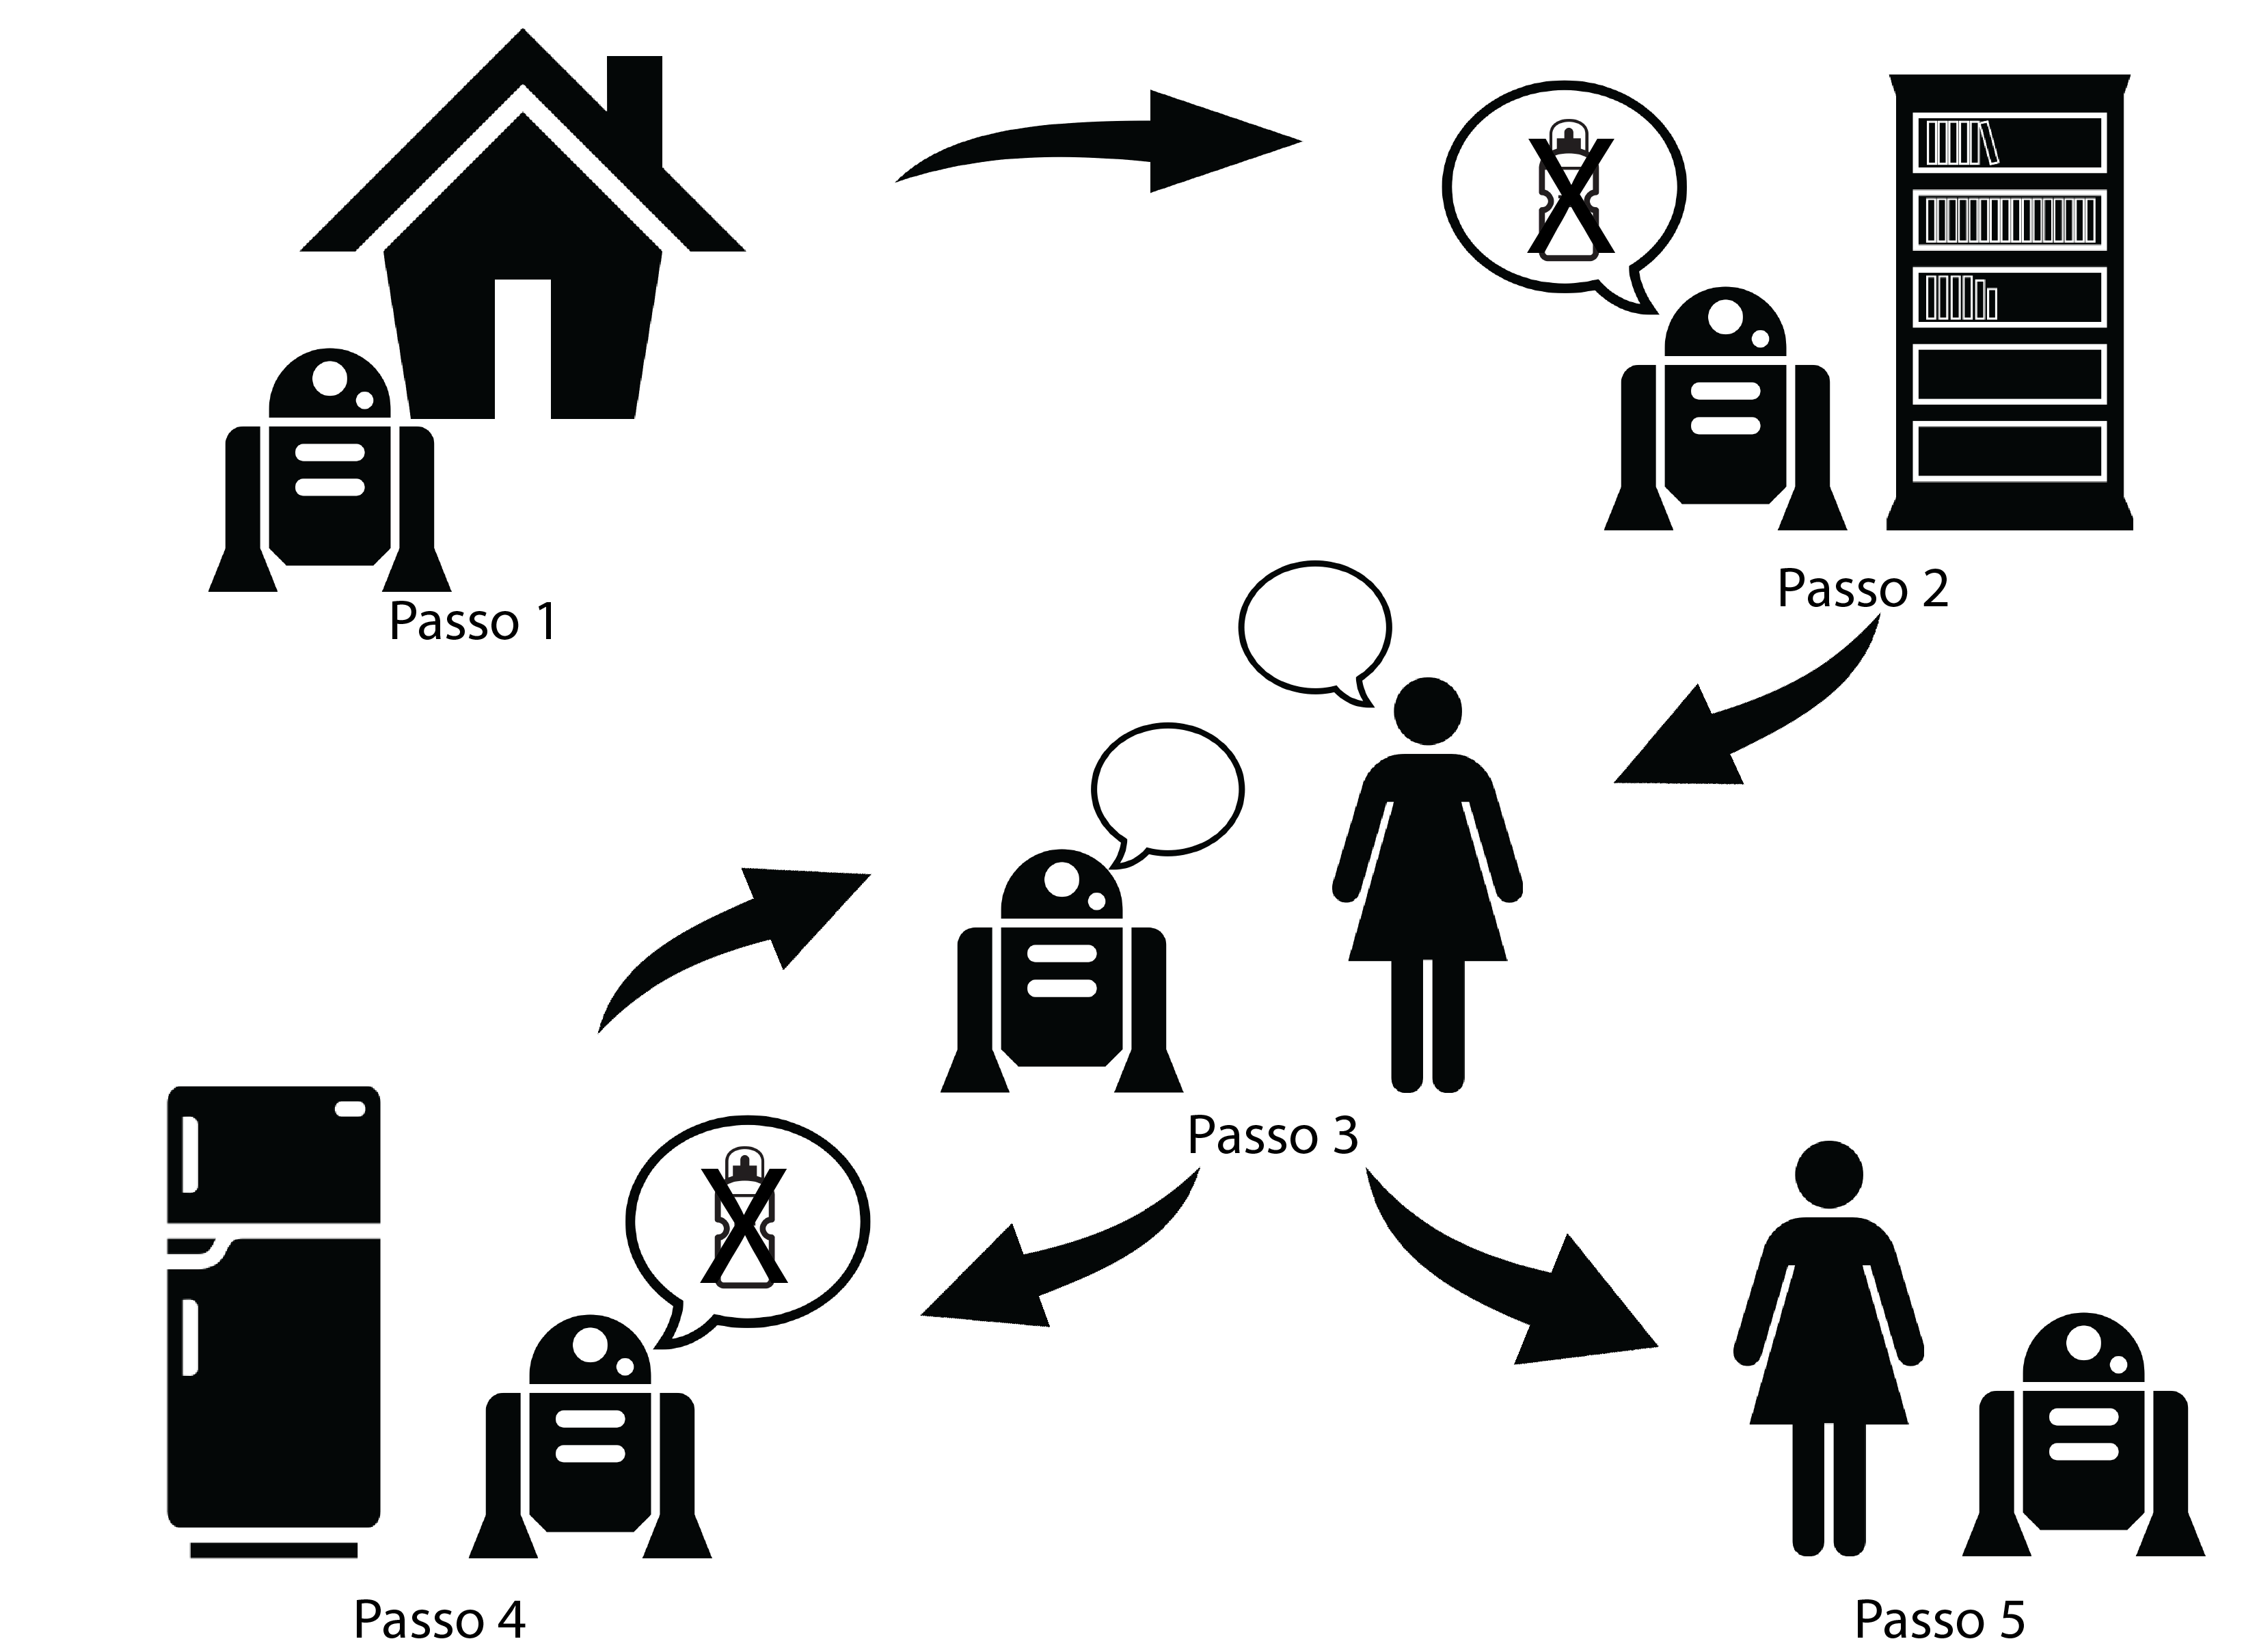
\includegraphics[width=\textwidth]{contexto-uso.png}
		\smallcaption{Fonte: o autor.}
		\label{fig:contextouso}
	\end{minipage}
\end{figure}

O cenário apresentado na figura~\ref{fig:contextouso} ilustra uma situação onde o robô entra em sua casa (passo 1) e vai até a estante onde ele deixou uma garrafa. A garrafa não está mais no local que ele deixou (passo 2), então ele vai até a pessoa que convive com ele no ambiente da casa. Ao interagir com a pessoa, o robô pergunta se ela viu a garrafa e recebe uma resposta negativa (passo 3). Na sequência, o robô procura pela garrafa em outro cômodo da casa, onde também não encontra (passo 4). O robô então retorna ao encontro da pessoa, e solicita a ajuda para procurar pela garrafa (passo 3). Como última etapa, a pessoa atende o pedido e ambos saem para procurar pela garrafa (passo 5), finalizando assim o cenário.

Através dessa ilustração pode-se definir o contexto de uso desta tese, onde o robô realiza a aproximação de pessoas que convivem com ele dentro de uma casa. Essa aproximação é realizada com o objetivo de solicitar ajuda ao humano para encontrar um objeto que foi deixado em algum lugar da casa. Com as variáveis identificadas e o contexto de uso da tese definidos, é necessário realizar a especificação do projeto, considerando fatores de engenharia de \emph{software} e fatores humanos já que existe interação humano-robô.

\section{Especificando o Projeto de IHR}
\label{sec:projetoihr}
Nos capítulos sobre IHR (capítulo~\ref{cap:ihr}) e teoria de proximidade (capítulo~\ref{cap:proxemics}) são apresentados diversos trabalhos com o estudos sobre interação entre humanos e robôs em diversas áreas, como saúde, lazer, entreterimento e social. Porém, ao analisar os projetos feitos nos trabalhos relacionados, não existe nenhuma definição sobre a especificação do projeto, como requisitos, perfis de usuários atentidos com o projeto, entre outros. O contexto de uso, em alguns casos, é utilizado pois, o projeto tem um foco em uma determinada tarefa. Contudo, projetos sem especificações são difícies de serem reproduzidos, um vez que os robôs utilizados são bem específicos. Além de serem específicos, os robôs utilizados são construídos, nos laboratórios das universidades e centros de pesquisas, em parte das pesquisas. As demais pesquisas utilizam robôs como: Softbank NAO~\footnote{https://www.ald.softbankrobotics.com/en/robots/nao} e PR2~\footnote{http://www.willowgarage.com/pages/pr2/overview}, que são produzidos por empresas especializadas fazendo com que o projeto fique restrito a sua capacidade determinada pela fábrica.

Em engenharia de \emph{software} são estudados vários métodos que auxiliam na especificação do projeto. Nesses métodos são encontrados a contemplação de alguns princípios que garantem a reprodução, manutenção e evolução do projeto ao longo tempo. Os princípios de engenharia de \emph{software} não são vistos como regras, mas como boas práticas para o desenvolvimento do projeto~\cite{wazlawick:2013}. As boas práticas aplicadas em sistemas computacionais, também podem ser aplicadas no desenvolvimento de projetos de robôs.
